\documentclass[10pt]{article}
\usepackage[top=1.2in, bottom=0.7in, left=0.7in, right=0.7in]{geometry}
\usepackage{amsmath}
\usepackage{amsthm}
\usepackage{amssymb}
\usepackage{placeins}
\usepackage{marvosym}
\usepackage[usenames,dvipsnames,table]{xcolor}
\usepackage{colortbl}
\usepackage{booktabs}
\usepackage{graphicx}
\usepackage{framed}
\usepackage{setspace}
\usepackage{xspace}
\usepackage[labelfont=bf]{caption}
\usepackage{verbatim}
\usepackage{paralist}
\usepackage{algorithm}
\usepackage{algpseudocode}
\usepackage{wrapfig}
\usepackage[font=footnotesize,labelfont=bf,justification=justified,singlelinecheck=false]{caption}
\usepackage{titlesec}
\usepackage{natbib}
\usepackage{longtable}
\usepackage{tabularx}
\usepackage{tabulary}
\usepackage{multirow}
\usepackage{lipsum}
\usepackage{mathpazo}
\usepackage{authblk}
\usepackage{nameref}
\usepackage{cancel}
\usepackage{commath}
\usepackage{xspace}
\usepackage{dsfont}
\usepackage{cuted}
\usepackage{fancyhdr}
\usepackage{hyperref}
\newcommand{\varB}[1]{{\operatorname{\mathit{#1}}}}

% distance between columns
\setlength{\columnsep}{3ex}

% section rules
\titleformat{\paragraph}[runin]
{\normalfont\itshape}
{\theparagraph}{}{\noindent}[.---]

\titlespacing{\paragraph}{0pt}{3.25ex plus 1ex minus .2ex}{0em}

\titleformat{\section}
  {\centering\scshape}{\thesection}{1em}{}

\titleformat{\subsection}
  {\centering\itshape}{\thesubsection}{1em}{}

% bibliography settings

% header
\pagestyle{fancy}
\fancyhf{}
\fancyhead[RO,LE]{\thepage}
\fancyhead[C]{\scshape VETR ET AL.---Appendix 2}

% Title %

\title{\vspace{-2.5cm}Appendix 2}
\author{}
\date{}

\begin{document}

\maketitle{}

\section*{More Efficient Proposals Over Correlation Matrices}

\section{Motivation}

Correlation matrices are a special case of covariance matrix. They have all the latter's properties, including symmetry and positive semi-definiteness (PSD), in addition to the requirement of a unit diagonal. In Bayesian inferential contexts involving covariance matrices, it is common to factor covariance matrix $C$ into the matrix product $SRS$, where $S$ is a diagonal matrix of standard deviations and $R$ is a correlation matrix. Priors can then be specified on these components separately. Under the phylogenetic multivariate Brownian motion model, the rate matrix is a covariance matrix, describing the shape of the multivariate normal distribution --- scaled multiplicatively by the branch length --- from which displacements to the location of some vector of traits is drawn.

A problem arises when making proposals to correlation matrices during the Metropolis-Hastings algorithm \citep{hastingsMonteCarloSampling1970} used to numerically approximate the Bayesian joint posterior distribution of model parameters. The problem involves the PSD constraint, which with increasing matrix dimensionality rapidly narrows the window of viability available to each correlation coefficient, conditional on the values observed at all other positions of the correlation matrix. This is implied by the narrowing marginal distribution of each coefficient in samples from an LKJ distribution, which can be described by a beta distribution stretched into the (-1,1) range with shape parameters $\eta -1 + D/2$, where $D$ is the dimension of the correlation matrix. It can also be demonstrated experimentally by sampling a correlation matrix from a flat LKJ distribution ($\eta = 1$), selecting one of its off-diagonal elements, and identifying the magnitude of the interval about that element for which the PSD condition is preserved. Averaging across many replicates, we obtain an estimate of the expected interval over which proposals to individual elements of a correlation matrix may be made for matrices of a given size, which we summarize graphically (Figure \ref{fig:expWiggleRoom}).

As this interval shrinks, the Metropolis-Hastings algorithm slows tremendously with respect to its mixture over the posterior distribution of correlation matrices if naive proposal distributions are used that do not respect the constraint of positive semi-definiteness. Additionally, the number of parameters to be estimated increases quadratically with the dimension of the correlation matrix, as a correlation matrix of dimension \textit{n} has $(\textit{n}$ choose $2)$ off-diagonal elements. And tests for positive-semidefiniteness --- for example, involving eigendecomposition and the surveyance of positive eigenvalues --- can themselves become quite computationally cumbersome, especially at high dimensionality. As such, approaches that rely on the rejection of invalid proposals must either sample from more and more conservative distributions over increasingly many elements of the correlation matrix, or else make tremendously more proposals over the course of the MCMC.

Here, we describe a proposal distribution over correlation matrices that makes proposals to multiple correlation parameters simultaneously and is guaranteed to sample from the PSD space. It is asymmetric, and our description therefore also entails the calculation of forward and backward proposal probabilities. In addition, it is tunable on a per-trait-index basis, allowing for the optimization of acceptance probabilities contingent upon the narrowness of the target distribution. Finally, we describe its implementation with respect to the Cholesky factor of the correlation matrix, which is a commonly used internal representation of a correlation matrix for the purpose of computational efficiency (e.g. in transforming tip characters or specifying non-centered parameterizations in Gaussian Process Regression). The proposal distribution also samples a new Cholesky factor in $O(n^2)$ time complexity, removing the need to perform a more costly $O(n^3)$ Cholesky factorization. One minor complication of the below described proposal distribution involves its return of a Cholesky factor corresponding to a permuted correlation matrix, rather than one with the original row and column indexing. In our implementation, an optional argument can be toggled to return to the original order at the cost of some of the aforementioned efficiency. Instead, we prefer to permute the (e.g. multivariate normal) data whose density is being calculated, a much more efficient procedure that nevertheless requires slightly more bookkeeping.

Following our description of the proposal distribution, we conduct a short validation of its performance, first using it to sample via the Metropolis-Hastings algorithm from a flat LKJ distribution --- uniform over all correlation matrices --- and comparing these samples to those drawn directly from the LKJ. Then, we use the proposal distribution to approximate a more informative distribution: the posterior distribution of the correlation matrix of a 10-dimensional multivariate normal random variable whose means and variances are known, conditional on 50 samples from that distribution and an LKJ($\eta = 1$) prior. We compare these to the same distribution independently approximated through more innocuous means: a uniform sliding window proposal over all choose(10, 2) pairwise elements of the correlation matrix. The former is run for 1E7 iterations and the latter for 5E7, with thinning occurring at an interval of 1E3 and 5E3, respectively. The first 20\% of each chain is discarded as burn-in, and automatic tuning is performed across 50 sub-rounds of burn-in to target a per-trait (in our novel proposal distribution) and per-correlation (in the uniform sliding window proposal distribution) acceptance probability of 0.234 \citep{robertsWeakConvergenceOptimal1997}. In practice, this resulted in acceptance probabilities ultimately falling in the interval (0.20, 0.24).

\clearpage

\section{Description}

The proposal distribution was inspired by the \textit{extended onion method} of the \citeyear{lewandowskiGeneratingRandomCorrelation2009} paper by Lewandowski, Kurowicka, and Joe for sampling from the eponymous LKJ distribution. In this algorithm, the Cholesky factor of a correlation matrix is built iteratively up to the desired dimensionality \textit{n}, one layer at a time, as one might grow an onion. Our proposal distribution simply unravels the last step of the extended onion method, corresponding to the construction of the correlations of the \textit{n}th variable with the remaining \textit{n} - 1 variables of the \textit{n} x \textit{n} correlation matrix. In the extended onion method, this final column of the upper Cholesky factor \textit{U} is constructed through sampling a single beta distributed random variable \textit{y} from a beta(\textit{n}/2, $\eta$), and a vector $u=(\textit{u}_{1},...,\textit{u}_{\textit{n-1}})$ uniformly sampled from the surface of an \textit{n}-dimensional hypersphere. The \textit{u} are then rescaled by the square root of \textit{y} to form the first \textit{n} - 1 elements of the column of \textit{U}. The square root of (1-\textit{y}) then forms the last entry of that column, ensuring unit length. 

Working backwards, we can straightforwardly identify the unique \textit{y} and \textit{u} necessary to produce some current \textit{U}, conditional also on its (\textit{n} - 1) x (\textit{n} - 1) submatrix. We can then resample these values centered on these targeted states --- disallowing any room around them will reproduce \textit{U}, and resampling from \textit{y} $\sim$ beta(\textit{n}/2, $\eta$) and \textit{u} $\sim$ uniform on the unit hypersphere will generate a sample from the conditional LKJ($\eta$). Between these extremes, we can resample \textit{$y^\prime$} from within a window of tunable width \textit{w} centered around the target \textit{y} in proportion to its probability density in beta(\textit{n}/2, $\eta$) through the cumulative distribution and quantile functions of the beta distribution, with forward and backward proposal probabilities equal to the cumulative probability contained within each window centered on the forward state \textit{y} and backward state \textit{$y^\prime$}, i.e. found by integrating the beta probability density function between each set of bounds, which has positive density in (0,1) and zero density elsewhere. Resampling \textit{$u^\prime$}, meanwhile, can be accomplished by sampling \textit{n} - 1 normal random variables with mean = \textit{u} and variance = tuning parameter \textit{v}, and then rescaling this vector to unit length. By rescaling, we permit infinitely many samples from the aforementioned normal distributions to correspond to the same \textit{$u^\prime$}, all falling on the vector stretching from the origin through \textit{$u^\prime$}. Forward and backward proposal probabilities can be obtained by integrating along this vector the multivariate normal probability distribution function with mean equal to the target state \textit{u} or \textit{$u^\prime$} and covariance matrix diagonal with entries \textit{v}. However, symmetry in the proposal distributions results in these integrals evaluating to the same value, and so the proposal ratio for this step can be set to 1.

As yet, the above proposal distribution samples only correlations of the final row and column of some correlation matrix R = $U^{T}U$. Its aggressiveness is controlled by two tuning parameters, \textit{w} and \textit{v}, though in practice we find that setting \textit{w} to some small value, such as 0.1, and tuning only \textit{v} is sufficient to achieve desired acceptance probabilities on moderately informative target distributions, such as those used in the second experiment below. For more informative target distributions, tuning \textit{w} may also become necessary. Working on only the last dimension of \textit{U} can be inefficiently accommodated by recomposing R, permuting, and refactoring. However, we can more cheaply remain in upper Cholesky form through two $O(n^2)$ steps, a rank-one update and downdate involving a series of Givens rotations, implemented in the R-package \textit{mgcv} \citep{woodPackageMgcv2015} as the function \texttt{choldrop}, followed by the solution of a triangular system of equations to reinsert the removed column in the final place, accomplished with base-R \citep{rcoreteamLanguageEnvironmentStatistical2013} function \texttt{backsolve}. To return the Cholesky factor to its original order, this procedure could be performed \textit{n - i} times, where \textit{i} is the index of the character deleted and reinserted. This is still more efficient than Cholesky factorization, but up to \textit{2n} times more costly than the small burden of permutation index bookkeeping. 

\clearpage

\section{Validation}

Having implemented this proposal distribution in R, we seek to validate its performance in simulation, first by sampling uniformly from the space of correlation matrices by setting the acceptance probability to the ratio of proposal probabilities, implicitly sampling from an LKJ(1) with dimension 10. After having done so, we sample directly and independently from the analytical distribution, and visually inspect quantile-quantile plots of the marginal correlations and matrix determinants (Figure \ref{fig:priorSamplingResults}).

Noting that these fall along the 1-to-1 line, we move on to explore sampling from a more tightly constrained distribution of correlation matrices, that defined by the joint posterior distribution of correlation matrices of a multivariate normal random variable with mean and variances known and equal to 1 and 10 x 10 correlation matrix drawn from an LKJ($\eta = 1$) (Figure \ref{fig:sample10x10CorrMatrix}).

Specifically, this distribution represents the compromise between our flat LKJ($\eta = 1$) prior and the information contained in 50 samples from the above described multivariate normal, with target distribution density equal to the probability densities of our 50 draws with correlation matrix sampled and means and variances fixed. Comparing the samples obtained using the novel proposal distribution to those using the conventional sliding window, we first visually examining marginal trace plots and histograms and find that they closely overlap. Following that, we construct a similar figure as above, visualizing quantile-quantile plots and covariance patterns in both sets of samples and noting that they hew close to the 1-to-1 line, indicating that the same distribution is being sampled in both cases (Figure \ref{fig:posteriorSamplingResults}).

Then, we coerce both arrays of correlation matrices to \texttt{mcmc.list} objects and evaluate Gelman and Rubin's Convergence Diagnostic \citep{gelmanInferenceIterativeSimulation1992} in the R package \textit{coda} \citep{plummerCODAConvergenceDiagnosis2006}, finding for all pairwise correlations upper 95\% confidence interval values of 1.00 and a multivariate \(\hat{R}\) of 1. Effective sample sizes (ESS) of marginal correlations for both chains together ranged between 3,793 and 14,483, though much of those were from the chain using our novel proposal distribution, whose ESS ranged between 3,279 and 8,052, rather than from the sliding window chain, whose ESS ranged between 458 and 6,482, despite the latter having been tuned to have elementwise acceptance probabilities of 0.234 and being run for fivefold the number of iterations. 

\clearpage

\section{Conclusion}

Thus, we have described, implemented, and validated a novel proposal distribution for correlation matrices. Our validation used a relatively small 10 x 10 correlation matrix --- much greater improvements would be found with matrices of higher dimensionality. Often, Cholesky factorization counts among the most computationally steps of phylogenetic likelihood calculation in multivariate Brownian models, and circumventing this step by making proposals directly to the Cholesky form should enable tremendous gains to efficiency when performing inference of the character evolutionary processes governing the evolution of multiple traits. Even if one desires proposals directly on correlation matrices, making smarter proposals to multiple correlations simultaneously without the need for expensive PSD checks and rejection sampling should offer a substantial improvement to the use of more naive proposal distributions that do not intrinsically respect their constraints and properties.

\clearpage

\section{Figures}

\begin{figure*}[h]
\centering
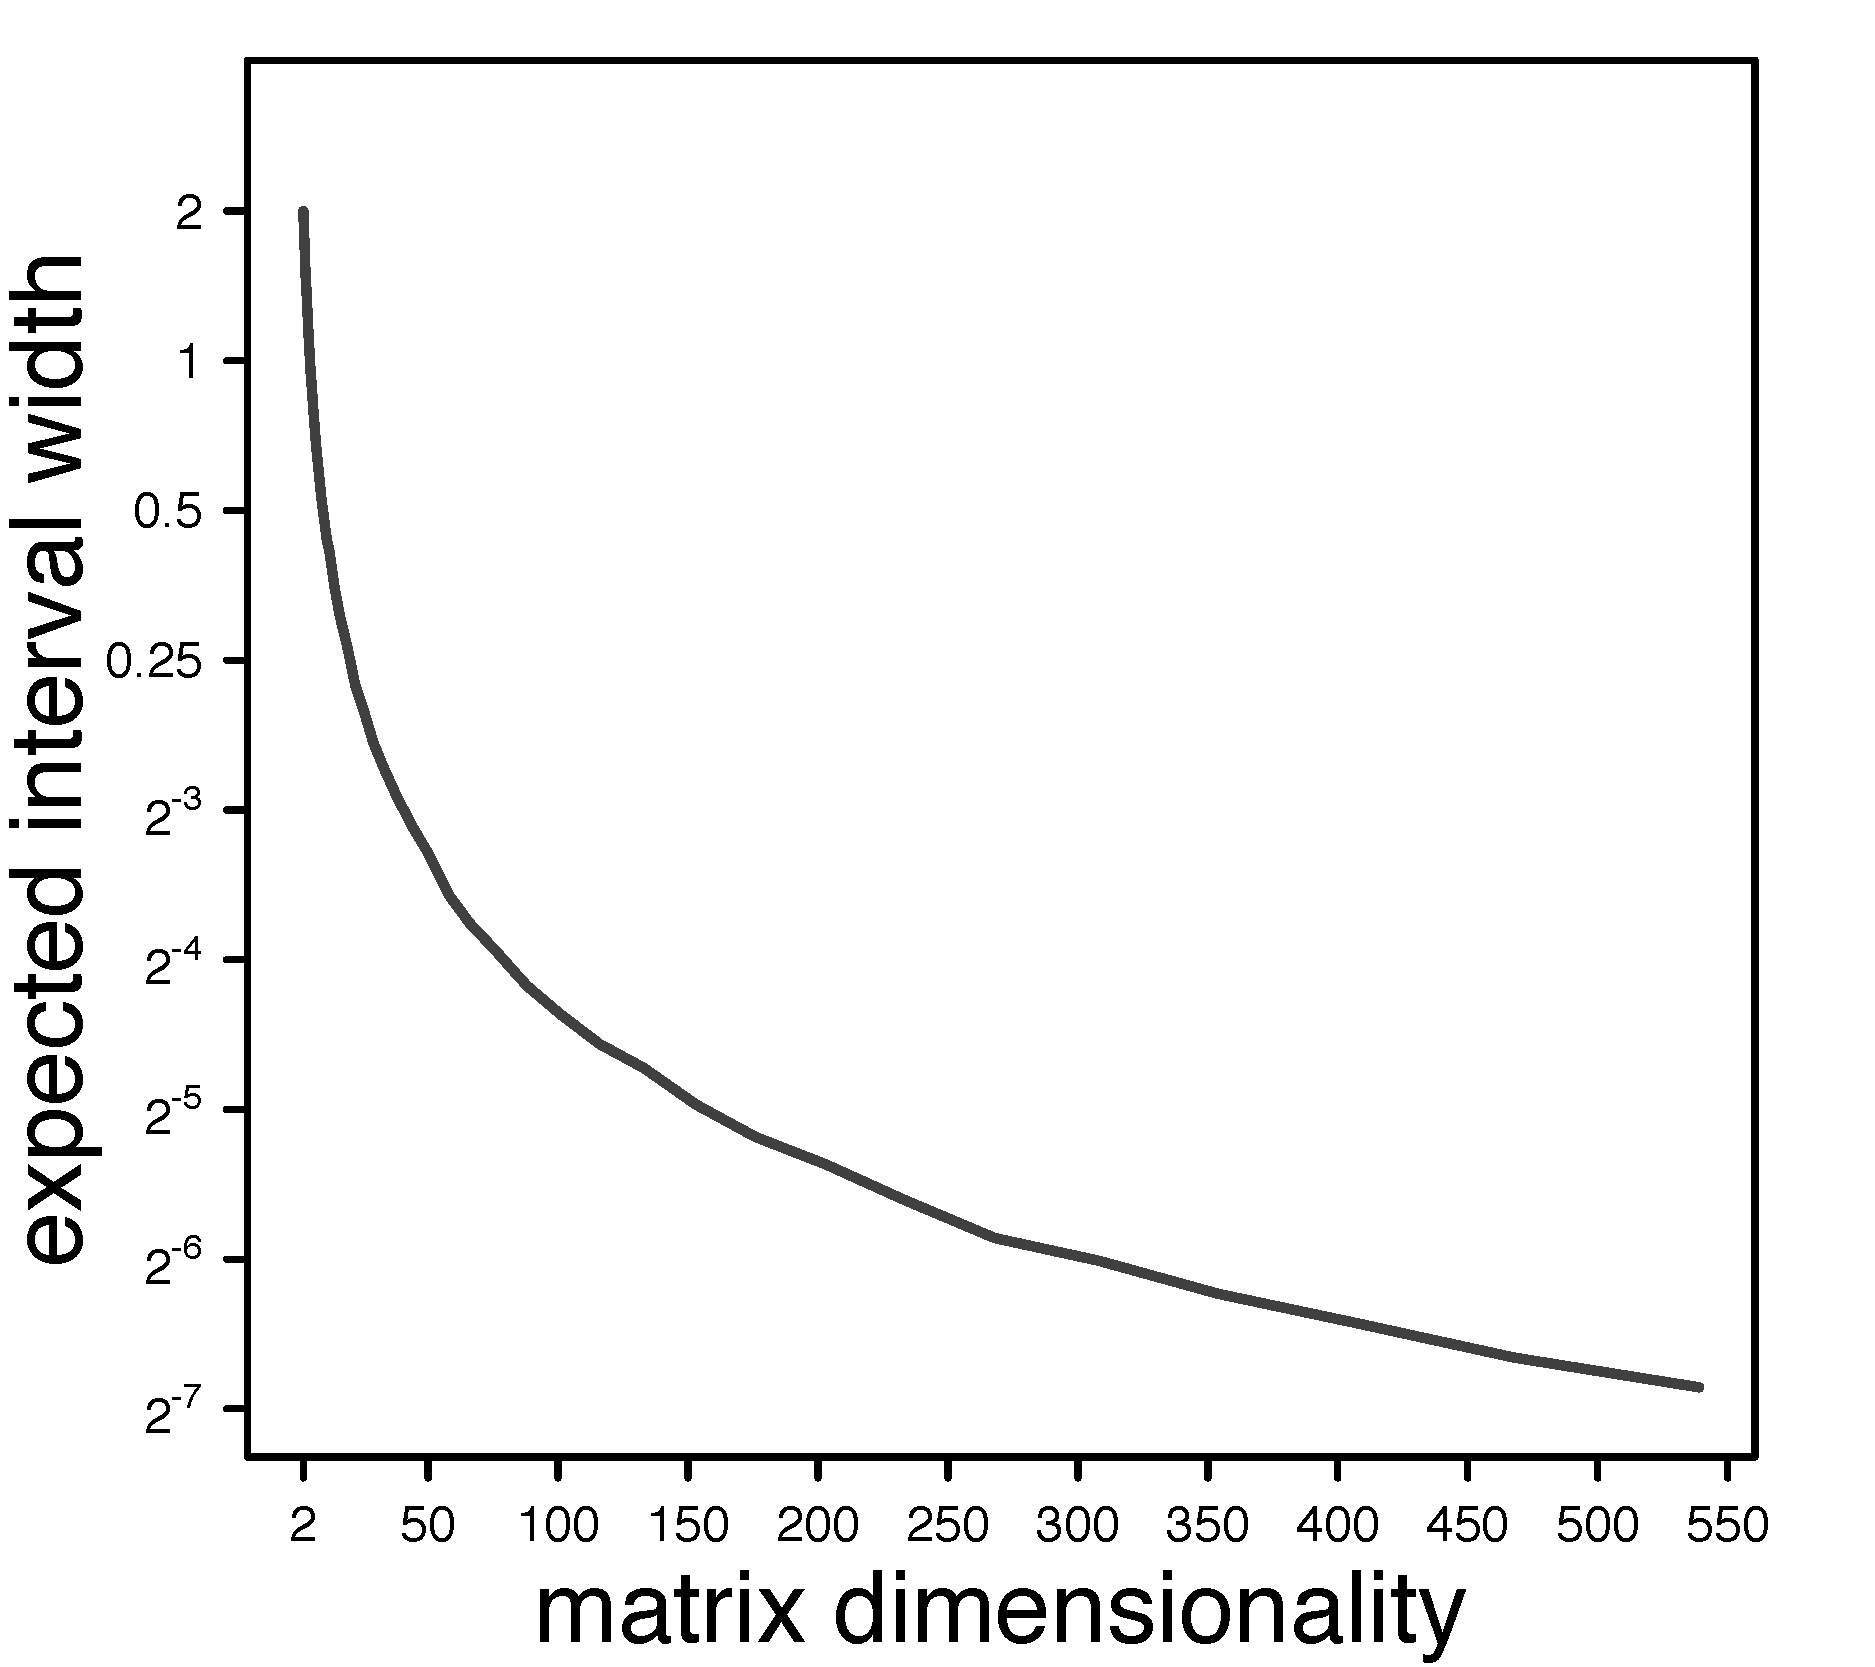
\includegraphics[width=145mm]{figures/expected_wiggle_room.pdf}
\caption[Expected Valid Sliding Window Width for Correlation Matrix Across Dimensions]{Depicting the relationship between how much space, in expectation, is available in a random correlation matrix of given dimensionality for valid proposals to marginal correlation coefficients. Quantities approximated using Monte Carlo simulation using samples from an LKJ($\eta = 1$). A random correlation coefficient was then chosen and perturbed in both directions by increasing amounts until the PSD constraint was violated. \label{overflow}
\label{fig:expWiggleRoom}}
\end{figure*}

\begin{figure*}[h]
\centering
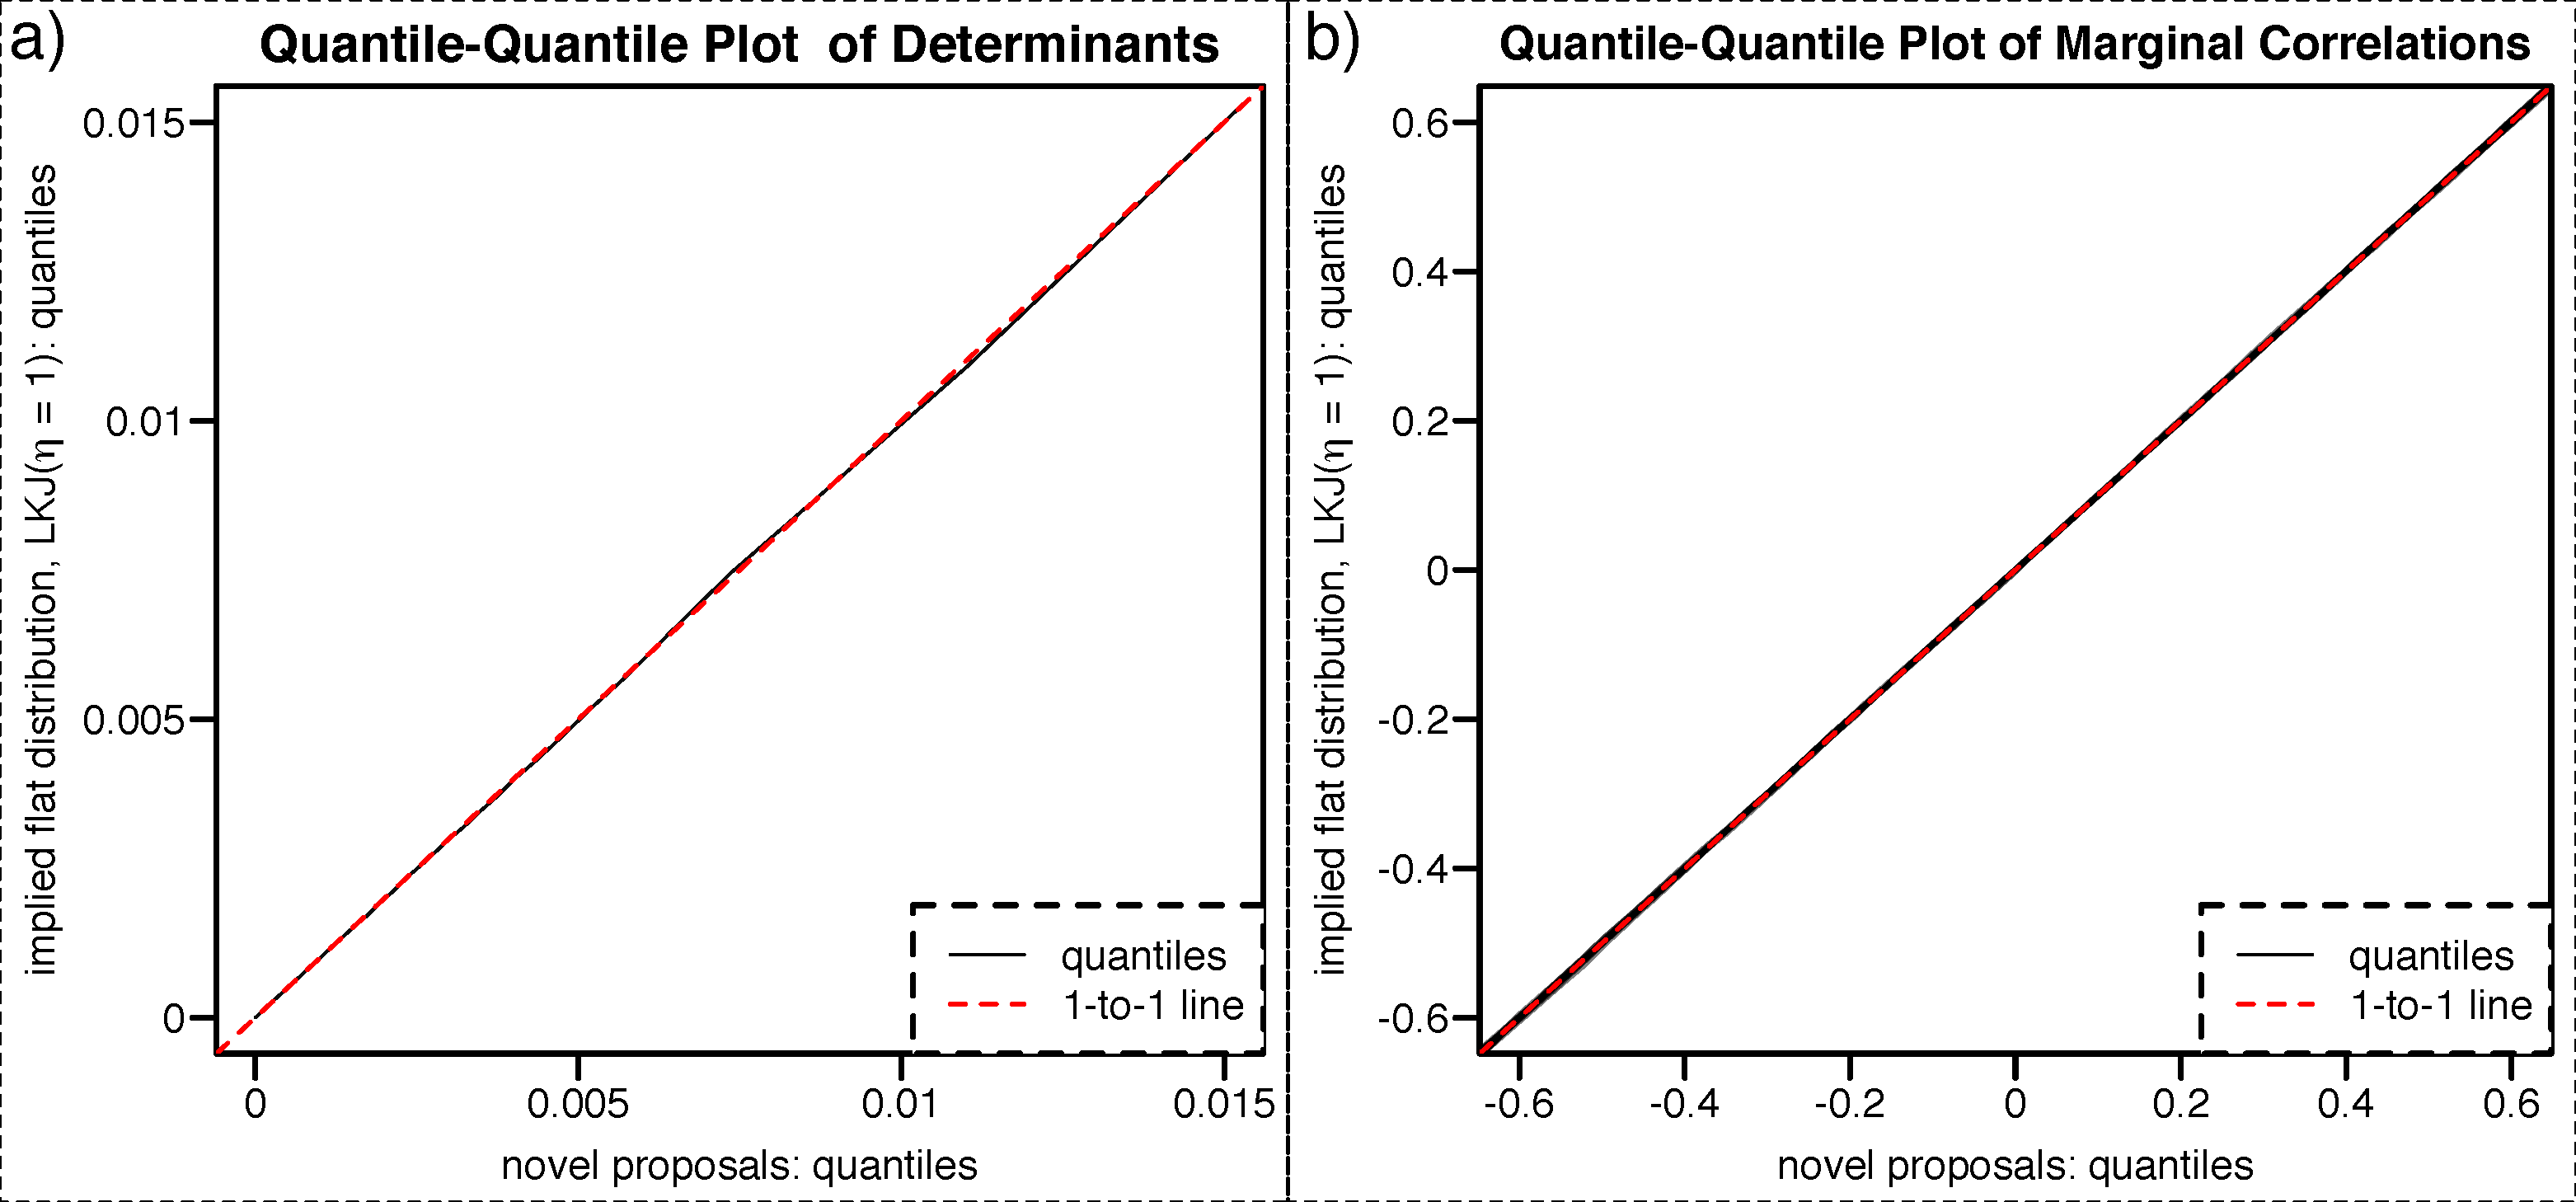
\includegraphics[width=145mm]{figures/app_lkj1_samples.pdf}
\caption[Sampling from the Prior with a Novel Proposal Distribution]{Depicting an initial experiment in the correct specification of the novel proposal distribution described herein. Target distribution density ratio was set to 1, implicitly sampling 10 x 10 correlation matrices from an LKJ($\eta = 1$). Samples were then generated from this distribution directly, and the quantiles of marginal correlation coefficients and matrix determinants compared. \label{overflow}
\label{fig:priorSamplingResults}}
\end{figure*}

\begin{figure*}[h]
\centering
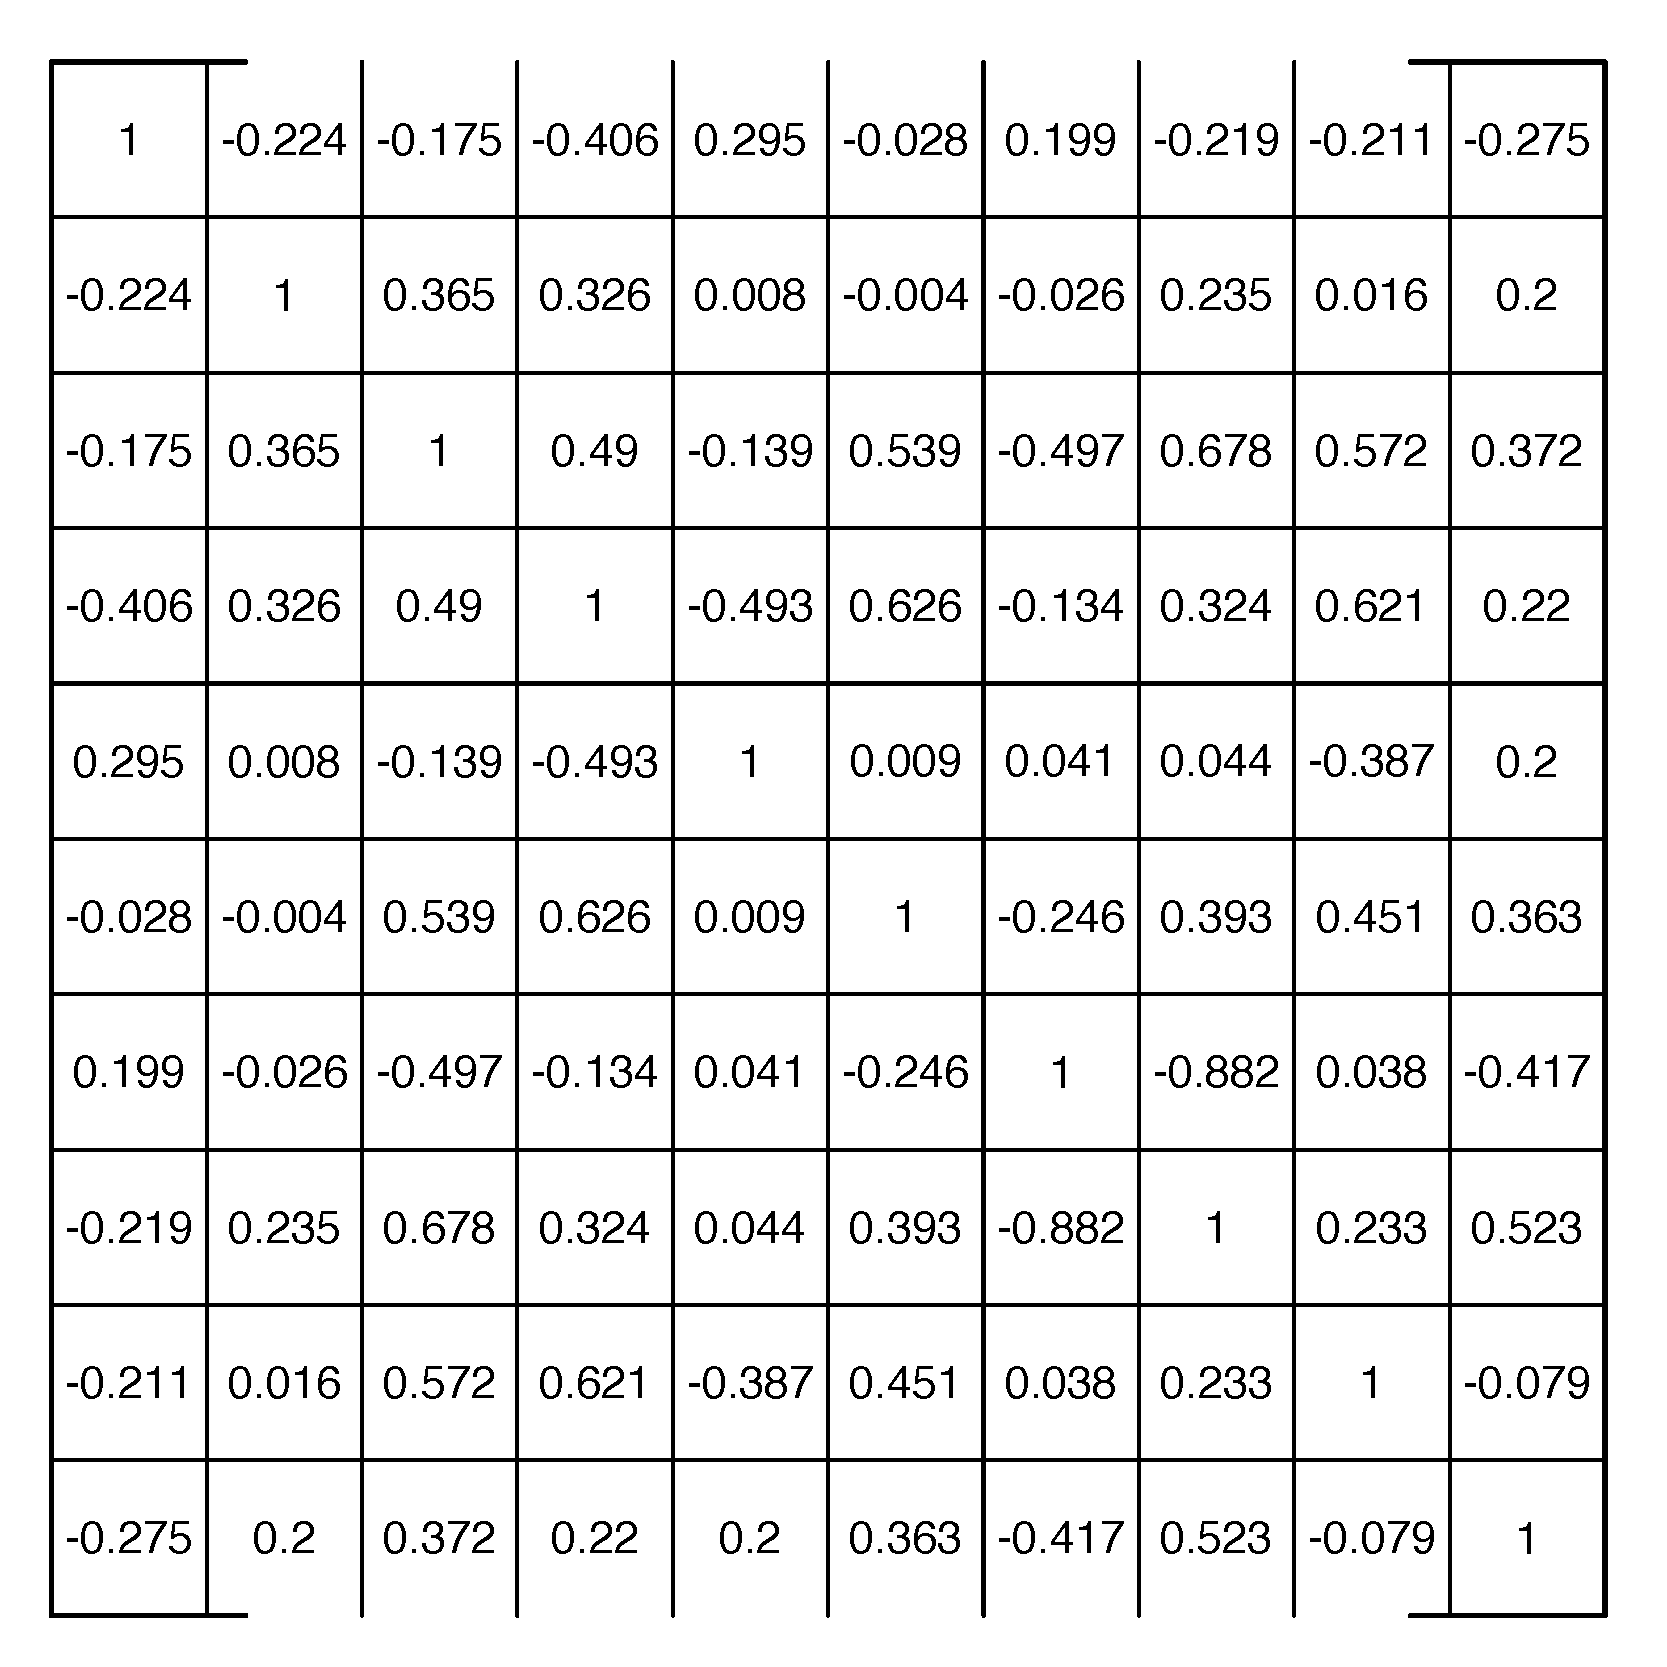
\includegraphics[width=100mm]{figures/appendix_correlationmatrix.pdf}
\caption[10 x 10 Correlation Matrix Used in Simulation Experiment]{The 10 x 10 covariance matrix used to generate samples from a multivariate normal distribution in the ``informative target distribution" experiment. Generated by sampling from an LKJ($\eta = 1$) distribution after calling \texttt{set.seed(1)} in \textit{R}. \label{fig:sample10x10CorrMatrix}
\label{overflow}}
\end{figure*}

\begin{figure*}[h]
\centering
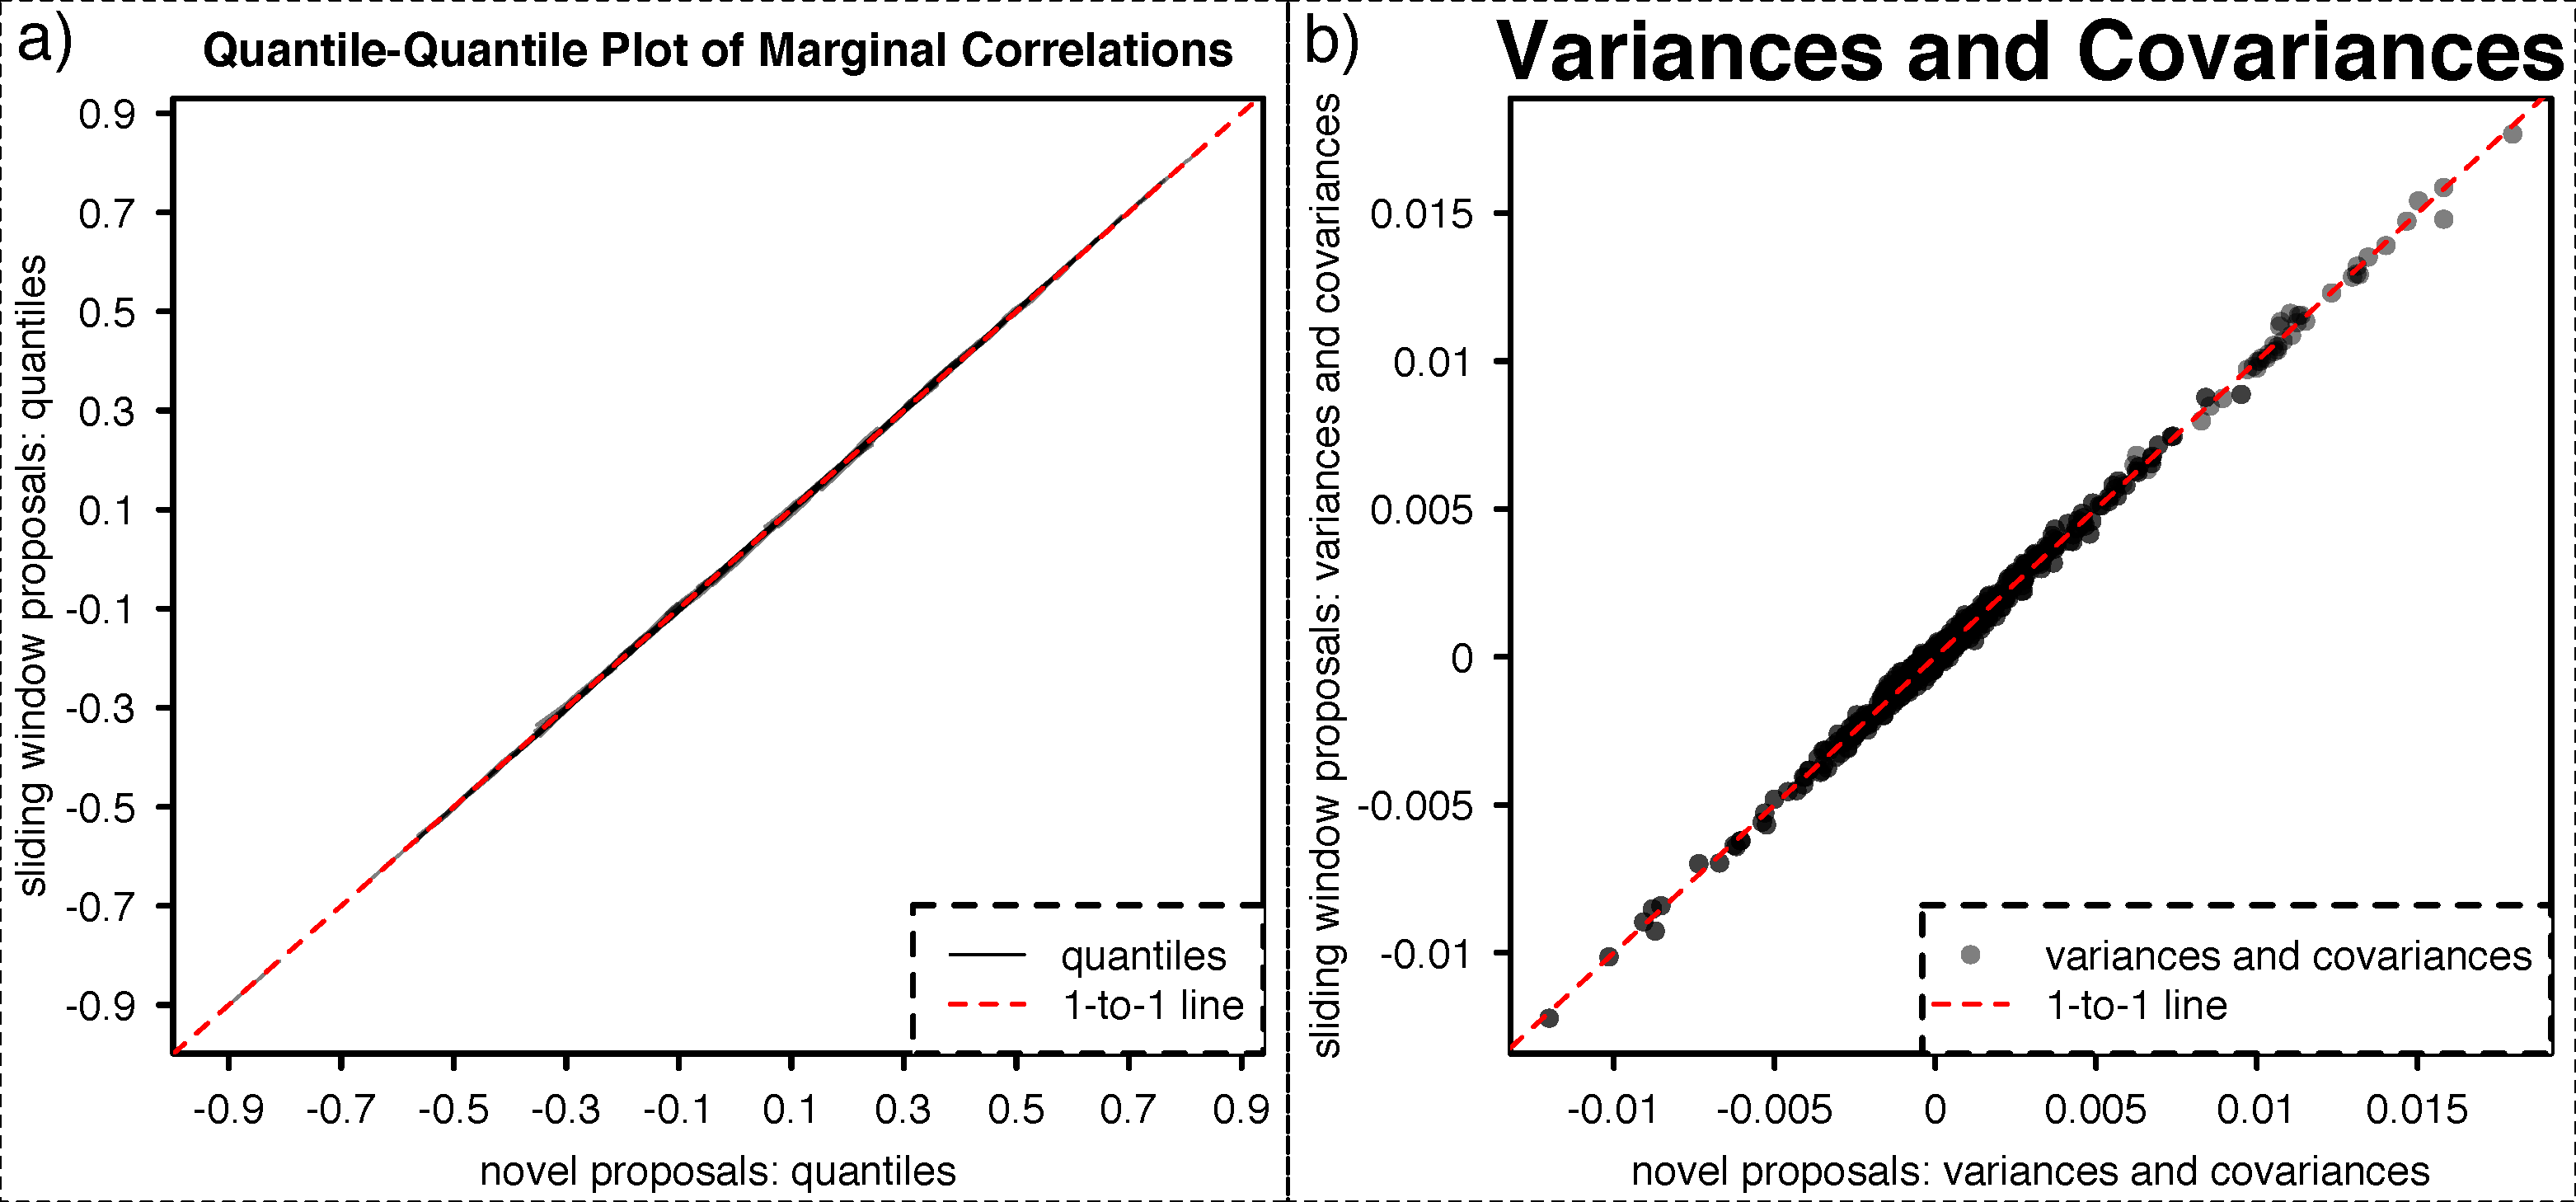
\includegraphics[width=160mm]{figures/app_corrs_2methods.pdf}
\caption[Sampling from the Posterior with a Novel Proposal Distribution]{A visual comparison of MCMC output obtained using both our novel correlation matrix proposal distribution and a more standard uniform sliding window proposal distribution. In a), quantiles of each marginal correlation coefficient are plotted. In b), the variances and covariances of each marginal correlation coefficient for both chains are plotted.
\label{fig:posteriorSamplingResults} 
\label{overflow}}
\end{figure*}

\end{document} %transformations to the determinant